\documentclass{article}
\usepackage[utf8]{inputenc}
\usepackage{graphicx}

\author{Bijan Varjavand}
\title{Solo Lab Write-up}

\begin{document}

\maketitle
1. Characterize the microstructure of materials using optical microscopy\\
a. mount, polish, etch inorganic\\
b. knowledge of optical microscopy\\
c. analysis of grain size and phase distribution\\

2. characterize crystal structure with xrd\\
a. knowledge of symmetric x-ray diff\\
b. analyze xrd scans for phases, planes, planar spacings, and lattice parameters, electronically and manually

\section{Introduction - The Unit Cell}

The unit cell has multiple different conformations. Examples include simple cubic(sc), body-centered cubic(bcc), and face-centered cubic(fcc).

\begin{figure}[h]
	\begin{minipage}{0.32\textwidth}
		\centering
		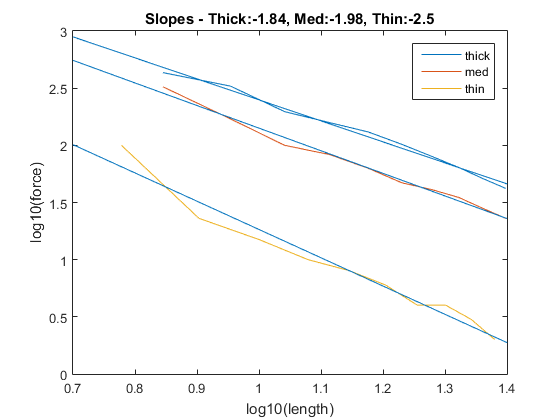
\includegraphics[scale=.3]{Lab1f1.png}
	\end{minipage}
	\begin{minipage}{0.32\textwidth}
		\centering
		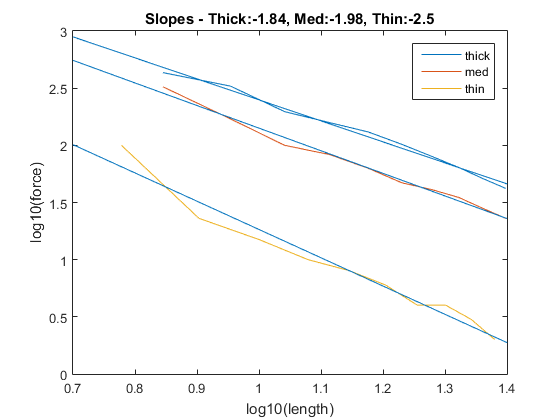
\includegraphics[scale=.3]{Lab1f1.png}
	\end{minipage}
	\begin{minipage}{0.32\textwidth}
		\centering
		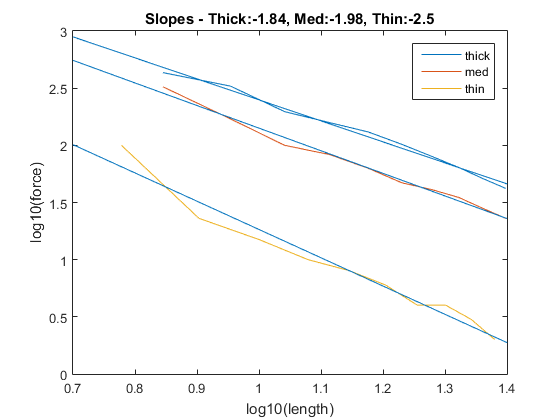
\includegraphics[scale=.3]{Lab1f1.png}
	\end{minipage}
	\caption{Left: SC, Mid: BCC, Right: FCC}
\end{figure}

One important aspect of a unit cell is the burgers vector and dense direction. These values indicate the direction of most dense packing. Notation for these dense direction is in miller indices (h, k, l, where hkl are orthogonal directional axes). Not only that, but due to symmetry of unit cells, the burgers vector is a family of h, k, and l values. For example, the family $\{1 1 0\}$ includes all hkl values that, when squares are added, equal 1. This is actually the burgers vector for BCC unit cells, and a few are shown below.

\begin{figure}[h]
	\centering
	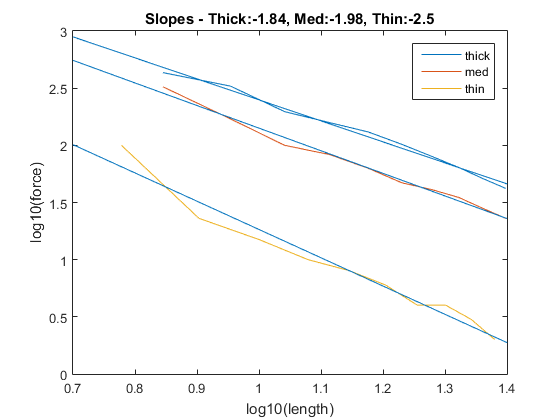
\includegraphics[scale=.3]{Lab1f1.png}
\end{figure}

The orientation of h, k, and l vectors are linked to each other within each grain. At the grain boundary, dislocation lines separate the slight change in orientation of h, k, and l vectors. These lines are visible to optical microscopy and can be counted - exactly the contents of this section of the lab.

\section{Optical Microscopy}

\subsection{Intro and prep}

Optical microscopy is a technique that uses light to view the sample at high magnification. The main method of generating images at such high magnifications are the use of multiple magnifying lenses as well as a light source. A diagram of the layout can be seen below along with a visual picture:

\begin{figure}[h]
	\begin{minipage}{.5\textwidth}
		\centering
		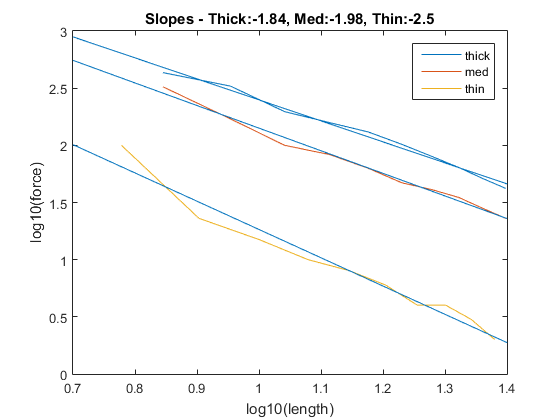
\includegraphics[scale=.3]{Lab1f1.png}
	\end{minipage}		
	\begin{minipage}{.5\textwidth}
		\centering
		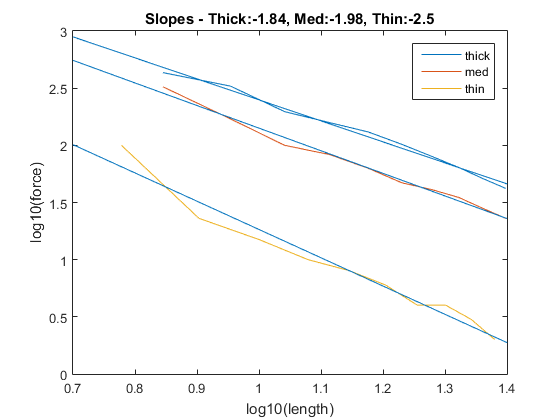
\includegraphics[scale=.3]{Lab1f1.png}
	\end{minipage}
\end{figure}

Preparing my samples to be viewed by the optical microscope was not trivial. The first step after acquiring my sample was to polish it. The complexity with polishing is that one can't use a grit too low or high. Grit too low will destroy the features of the sample, while grit too high polishes too inefficiently. Personally, I began with hand-polishing my sample on sand paper, smoothing edges and removing oxidation layers from the needed face. After that, I generated a puck of epoxy with the sample embedded inside. This puck was designed specifically to be fit into the polishing machine. This puck was then polished on the machine, and, using the software's predesigned polishing stages, was polished to an acceptable degree for viewing on the optical microscope.

\subsection{Procedure}

The specific microscope we used utilized the $\textbf{\_\_\_\_\_\_\_}$ software. The first step was to focus the microscope on a lower magnification setting and locate relevant features at acceptable quality (specifically avoiding scratching among other defects). blah. I generated these images, only showing the ones for annealed steel below. The data for the other materials can be easily found in the same directory as this pdf.

\subsection{Results and Observations}

\begin{figure}[h]
	\begin{minipage}{0.32\textwidth}
		\centering
		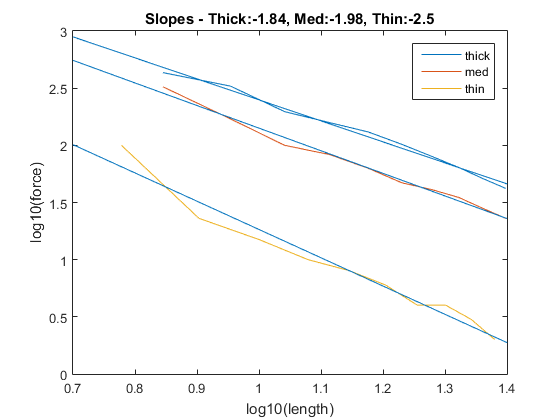
\includegraphics[scale=.3]{Lab1f1.png}
	\end{minipage}
	\begin{minipage}{0.32\textwidth}
		\centering
		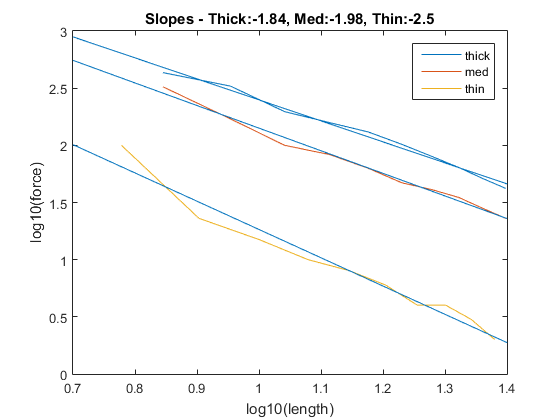
\includegraphics[scale=.3]{Lab1f1.png}
	\end{minipage}
	\begin{minipage}{0.32\textwidth}
		\centering
		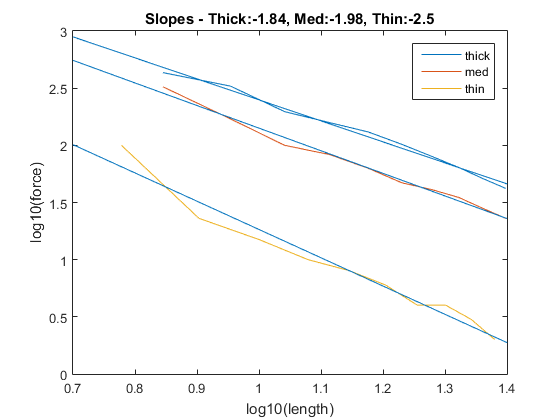
\includegraphics[scale=.3]{Lab1f1.png}
	\end{minipage}
	\caption{Left: SC, Mid: BCC, Right: FCC}
\end{figure}

The first step was to use the grain wizard to automatically calculate the grain index. blah. manual counting. ANSI standard.
$$equation$$
$$value = number$$

Description of relationship between calculated and found values.

\subsection{Error Analysis}

\section{X-Ray Diffraction}

\subsection{Intro}

X-Ray diffraction is a great thing that helps us.

\subsection{Procedure}

I did things.

\subsection{Results and Observations}

\begin{figure}[h]
	\begin{minipage}{.5\textwidth}
		\centering
		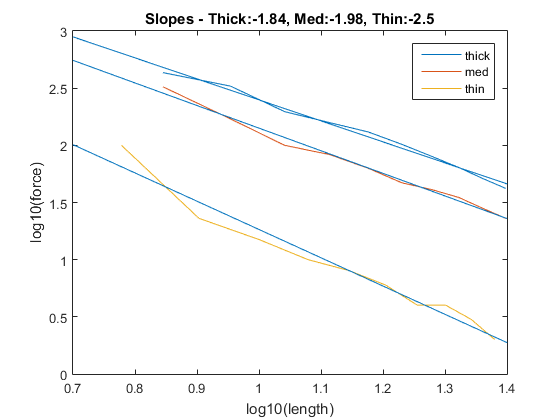
\includegraphics[scale=.3]{Lab1f1.png}
	\end{minipage}		
	\begin{minipage}{.5\textwidth}
		\centering
		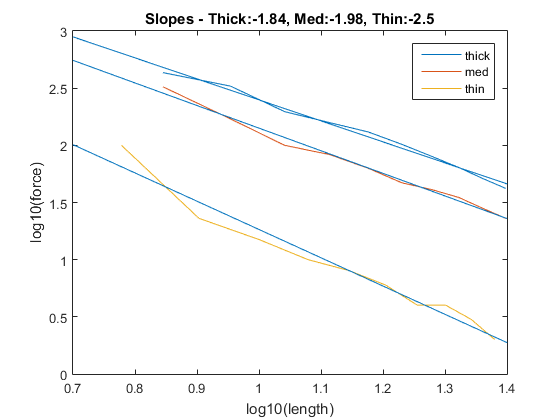
\includegraphics[scale=.3]{Lab1f1.png}
	\end{minipage}
\end{figure}

Wow thats amazing. Look it matches with what I thought.

\subsection{Error Analysis}


\end{document}